\documentclass[11pt,a4paper,german]{scrartcl}
%%%%%%%%%%%%%%%%%%%%%%%%%%%%%%%%%%%%%%%%%%%%%%%%%%%%%%%%%%%%%%%%%%%%%%%%%%
% Anpassungen f"ur das jeweilige "Ubungsblatt
\def\blnr{7}              % Blattnummer
\def\sdate{12.4.2019}    % Abgabedatum
\def\exnr{1}              % Nummer der ersten Aufgabe des aktuellen Blattes
%%%%%%%%%%%%%%%%%%%%%%%%%%%%%%%%%%%%%%%%%%%%%%%%%%%%%%%%%%%%%%%%%%%%%%%%%%
\usepackage{babel,theorem}
\usepackage{exscale}
\usepackage{amsmath,amsfonts,amssymb,dsfont}
\usepackage{a4wide}
\usepackage{epic,eepic}
\usepackage{graphicx} % einbinden von Grafiken mit \includegraphics
\usepackage{url}

\pagestyle{empty}
\parindent0em
\parskip1ex
\addtolength{\topmargin}{0cm}
\addtolength{\oddsidemargin}{0cm}
\addtolength{\textheight}{2cm}
\addtolength{\textwidth}{0cm}

% neuer Z"ahler f"ur die Aufgaben
\newcounter{aufgnr}
\setcounter{aufgnr}{\exnr}
\addtocounter{aufgnr}{-1}

% in enumerate-Umgebungen erst Kleinbuchstaben, dann kleine r"omische Zahlen
\renewcommand{\labelenumi}{(\alph{enumi})\,}
\renewcommand{\labelenumii}{(\roman{enumii})\,}

% Stil f"ur Definitionen, S"atze usw.
\theoremstyle{break}   % Titelzeile abgesetzt
\newtheorem{Satz}{Satz}
\newtheorem{Lem}{Lemma}
\newtheorem{Def}{Definition}
\theorembodyfont{\upshape}  % normaler Font f"ur Beispiel, Aufgabe
\newtheorem{Bsp}{Beispiel}
\newtheorem{aufg}[aufgnr]{Exercise}
\newenvironment{Exercise}[1][z*+]%
{\begin{aufg}}
  {\end{aufg}\vspace{1.5ex}}
\newtheorem{praktaufg}[aufgnr]{Aufgabe^*}
\newenvironment{PraktAufgabe}[1][]%  der optionale Param. muss in [[ .. ]]
{\begin{praktaufg}#1}
  {\end{praktaufg}\vspace{1.5ex}}

\newcommand{\zweifaelles}[3]{ \left\{ \begin{array}{ccc} #1 & \hspace{.8cm}  \mbox{ falls } #2 \, , &     \\[1ex]
                               #3 & \mbox{ sonst } &     \end{array} \right.     }
% Mathematische K"urzel
\def\R{\mathbb{R}}
\def\S{\mathbb{S}}
\def\C{\mathbb{C}}
\def\Q{\mathbb{Q}}
\def\N{\mathbb{N}}
\def\Z{\mathbb{Z}}
\def\P{\mathbb{P}}
\def\K{\mathbb{K}}
\def\O{{\mathcal O} }
\def\G{{\mathcal G} }
\def\T{{\mathcal T} }
\def\U{{\mathcal U} }

\newcommand{\arrl}{\begin{array}{l}}
\newcommand{\are}{\end{array}}
\newcommand{\arrc}{\begin{array}{c}}
\newcommand{\mza}{\begin{eqnarray}}
\newcommand{\mze}{\end{eqnarray}}
\newcommand{\dn}{\frac{\partial}{\partial n}}
\newcommand{\dny}{\frac{\partial}{\partial n(y)}}
\newcommand{\dd}[2]{\ensuremath{\frac{\partial^{#1}}{\partial #2}}}
\newcommand{\ov}{\overline}
\newcommand{\ma}{\mid\!}
\newcommand{\me}{\!\mid}
\newcommand{\impl}{\Rightarrow}
\newcommand{\sca}[3]{\ensuremath{(#1,#2)_{#3}}}
\newcommand{\nor}[2]{\ensuremath{\parallel\! #1 \!\parallel_{#2}}}
\newcommand{\ra}{\rightarrow}
\newcommand{\phin}{\varphi}
\newcommand{\diver}{\mbox{div}}

\def\eps{{\varepsilon}}
\def\i{{\sl i\;}}
\def\e{{\rm e}}
\def\D{{\rm D\;}}
\def\norm{|\!|\!|}

\DeclareMathOperator{\spann}{span}
\DeclareMathOperator{\cond}{cond}
\DeclareMathOperator{\round}{round}
\DeclareMathOperator{\supp}{supp}

\begin{document}

\parbox{0ex}{ \scalebox{.27}{  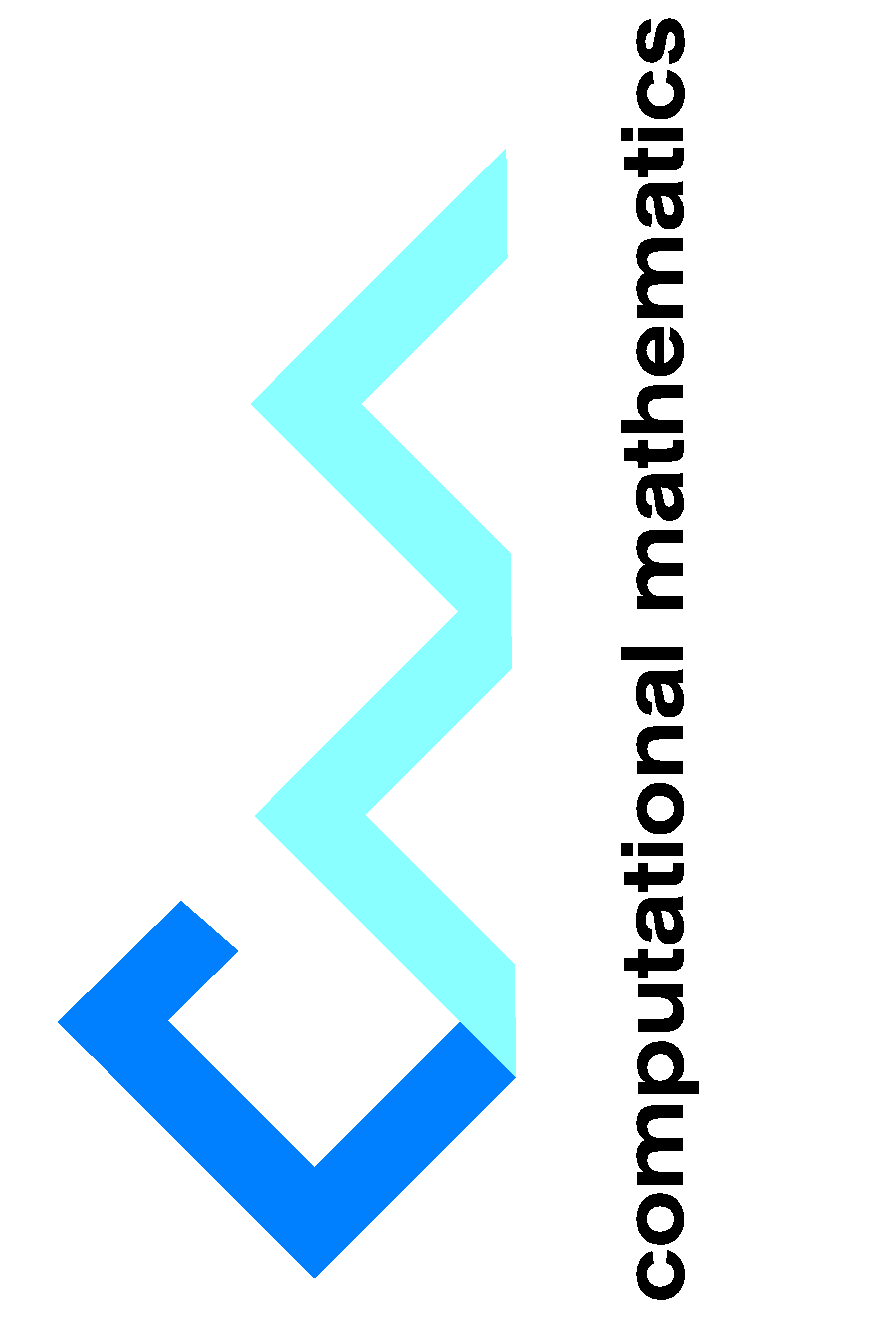
\includegraphics[width=.5\textwidth,angle=-90]{cm-logo2.eps} }   }   \\

\parbox{25ex}{
  Prof.~Dr.~S.~Sauter\\
  Institut f"ur Mathematik\\
  Universit"at Z"urich
  }
%
\rule[0cm]{0.cm}{.01cm}
\hfill  \parbox{0.6\textwidth}{
  {\sffamily\LARGE\bfseries Numerik I}
  {\sffamily\Large\bfseries \;\;--\;\; Homework \blnr }\\[1.5ex]
  Deadline: \sdate\ 13:00
  }
  
  
\vspace{10ex}

\textbf{Exercise 1} (6 P.) (Mixed taks) \\
We want to approximate
\begin{align*}
\int_{-1}^1 f(x)dx.
\end{align*}
\begin{enumerate}
\item Find nodes \(x_0,x_1,x_2 \in [-1,1]\) and weights \(w_0,w_1,w_2\) such that the quadrature 
\begin{align*}
Q(f) = w_0 f(x_0) + w_1 f(x_1) +w_2 f(x_2)
\end{align*}
has maximal degrees of exactness (Definition 6.5).
\item Implement the composed quadrature method derived in (a). Input: number of subintervals \(n\), values of \(f\) in the nodes.
\item Compare the convergence of the method with the Simpson's quadrature w.r.t. the same number of subintervals. 
\item What is the advantage of each of the two methods?
\end{enumerate}
\vspace{4ex}


\textbf{Exercise 2} (4 P.) (Theoretical task) \\
Construct a quadrature formula for the approximation of
\[
I\left(  f\right)  =\int_{0}^{1}\omega\left(  x\right)  f\left(  x\right)
dx\quad\text{with\quad}\omega(x)=x^{1/3},
\]
having maximum degree of exactness, which uses the information $f(0)$ and $ \int_0^1 f(x)dx$.

Derive an error estimate using the Peano kernels.
\vspace{4ex}

\textbf{Exercise 3} (4 Pkt.) (Theoretical task)\\
We define the monic Legendre polynomials $L_n(x)$ as the monic polynomials of increasing degree which are orthogonal with respect to the $L^2$-inner product $\int_{-1}^1 uv~ dx$. Show that the following 3-term recursion gives the Legendre polynomials.
\begin{eqnarray}
P_0 \equiv 1,  \quad 
P_1 = x, \quad & \nonumber \\ 
P_{i+1}= xP_i - \left ( \dfrac{i^2}{4i^2-1} \right ) P_{i-1} & \mbox{for } i=1,2,\ldots \label{3term}
\end{eqnarray}
Hint: 
We know from the lectures that the Legendre polynomials satisfy the 3-term recursion
\begin{eqnarray}
P_0 \equiv 1,  \quad  P_{-1}\equiv 0 \quad & \nonumber \\ 
P_{k+1}= (x-\alpha_k) P_k - \beta_k P_{k-1} & \mbox{for } k=1,2,\ldots \label{3term_manu}
\end{eqnarray}
$\text{with }\alpha_k=\frac{\left(xP_k(x),P_k(x)\right)}{\left(P_k(x),P_k(x)\right)}  \text{ and }  \beta_k=\frac{\left(P_k(x),P_k(x)\right)}{\left(P_{k-1}(x),P_{k-1}(x)\right)} .$


Use symmetry with respect to 0 to compute $\alpha_k$. For \(\beta_k\) use the equivalent formula for \(P_k\) given by
\begin{equation}
P_{k}\left(  x\right)  =\left(  -1\right)  ^{k}\frac{k!}{\left(  2k\right)
!}\left(  \frac{d}{dx}\right)  ^{k}\left(  \left(  1-x^{2}\right)
^{k}\right)  .\label{RF}%
\end{equation}
Use integration by parts (\(k\) times) and a trigonometric change of variables to compute $(P_k,P_k)$ and, consequently, to find the formula for $\beta_k$.
%Prove that $P_k$'s in \eqref{PkFormula} reduces the 3-term recursion in manuscript (page 58) to \eqref{3term}. \\


\end{document}